% =====================================================================
%  BUỔI 9 — TÀI LIỆU BUỔI HỌC (từ hoc-sinh/02-tai-lieu-buoi-hoc.md)
%  Sinh tự động bằng scripts/md2tex-chung.py — không sửa tay.
% =====================================================================
\documentclass[11pt, a4paper]{article}
% =====================================================================
%  CAE SHANGHAI — GÓI LỆNH DÙNG CHUNG CHO TÀI LIỆU LUYỆN THI CSCA TOÁN
%  Biên dịch bằng XeLaTeX. Mọi file .tex trong buổi học \input file này.
% =====================================================================

% ---------- NGÔN NGỮ & PHÔNG CHỮ ----------
\usepackage{fontspec}
\usepackage{polyglossia}
\setmainlanguage{vietnamese}
\setotherlanguage{english}

% Chữ Latin (Anh + Việt): TeX Gyre Termes — bản clone Times New Roman,
% đi kèm TeX Live, hỗ trợ đầy đủ dấu tiếng Việt.
\setmainfont{TeX Gyre Termes}
\setsansfont{TeX Gyre Heros}

% Chữ Hán: ưu tiên Source Han Serif SC (思源宋体) — chuẩn học thuật Trung Quốc.
% Nếu máy chưa cài, tự động dùng Songti SC (宋体, có sẵn trên macOS).
% Cả hai đều thuộc họ 宋体 nên diện mạo tài liệu không đổi.
\IfFontExistsTF{Source Han Serif SC}{
  \newcommand{\cjkfamilyname}{Source Han Serif SC}
}{
  \IfFontExistsTF{Songti SC}{
    \newcommand{\cjkfamilyname}{Songti SC}
  }{
    \newcommand{\cjkfamilyname}{Noto Serif CJK SC}
  }
}

% xeCJK tự chuyển font khi gặp ký tự Hán, không cần bọc \cjk{} thủ công.
% Đây là điều kiện bắt buộc: font Latin (TeX Gyre Termes) không có glyph chữ Hán,
% nếu không khai báo xeCJK thì mọi chữ Hán viết trần sẽ bị nuốt khỏi bản in.
\usepackage{xeCJK}
\setCJKfamilyfont{caehan}{\cjkfamilyname}[Scale=0.95]
\setCJKmainfont{\cjkfamilyname}[Scale=0.95]
\setCJKsansfont{\cjkfamilyname}[Scale=0.95]
\setCJKmonofont{\cjkfamilyname}[Scale=0.95]

% \cjk{} ép dùng font Hán trong ngữ cảnh cần thiết (ví dụ trong tiêu đề in đậm
% hoặc trong bảng có định dạng riêng). Dùng \CJKfamily chứ không phải tên font,
% vì tên font chỉ là văn bản — sẽ in ra chữ thay vì đổi font.
\newcommand{\cjk}[1]{{\CJKfamily{caehan}#1}}

% ---------- TOÁN HỌC ----------
\usepackage{amsmath, amssymb, amsthm, mathtools}
\usepackage{unicode-math}
\setmathfont{TeX Gyre Termes Math}

% ---------- BỐ CỤC TRANG ----------
% Lề phải chừa vùng an toàn của letterhead:
%   banner trên chiếm 0–19mm  → top tối thiểu 2,2cm
%   banner dưới chiếm 281–297mm → bottom tối thiểu 2,2cm
% Lề trên 2,6cm (26mm) để tiêu đề đầu trang không đè banner (banner hết ở 19mm).
\usepackage[a4paper, top=2.6cm, bottom=2.4cm, left=2.5cm, right=2.0cm]{geometry}
\usepackage{fancyhdr}
\usepackage{titlesec}
\usepackage{enumitem}
\usepackage{graphicx}
\usepackage{booktabs, array, longtable, tabularx}
\usepackage{xcolor}
\usepackage[most]{tcolorbox}
\usepackage[colorlinks=true, linkcolor=cae_blue, citecolor=cae_blue, urlcolor=cae_blue]{hyperref}

% ---------- BẢNG MÀU THƯƠNG HIỆU ----------
\definecolor{cae_blue}{RGB}{0, 51, 102}
\definecolor{cae_gold}{RGB}{196, 149, 60}
\definecolor{box_bg}{RGB}{245, 247, 250}
\definecolor{box_line}{RGB}{0, 51, 102}

% ---------- TIÊU ĐỀ MỤC ----------
% Đệm đầu trang: banner letterhead chiếm 0–19mm, mà lề trên là 22mm.
% \section* đầu trang (sau \clearpage) sát lề nên phải chừa thêm, nếu không
% sẽ đè lên banner.
\titleformat{\section}
  {\normalfont\large\bfseries\sffamily\color{cae_blue}}{\thesection.}{0.6em}{}
\titleformat{\subsection}
  {\normalfont\normalsize\bfseries\sffamily\color{cae_blue!85!black}}{\thesubsection}{0.6em}{}
\titlespacing*{\section}{0pt}{14pt}{6pt}
\titlespacing*{\subsection}{0pt}{10pt}{4pt}

% Tiêu đề không đánh số ở đầu trang: \section* sau \clearpage nằm sát lề trên
% nên đè lên banner letterhead. Dùng \vspace* ngay TRƯỚC \section* không đủ,
% vì titlesec chèn khoảng cách riêng. Cách chắc chắn là đệm bằng \null.
\newcommand{\sectiondautrang}[1]{\section*{#1}}

% Dạng bài dùng \subsection*{} nên cần định dạng riêng, đậm và có gạch chân màu
\titleformat{\subsubsection}
  {\normalfont\normalsize\bfseries\sffamily\color{cae_blue!85!black}}{\thesubsubsection}{0.6em}{}

% ---------- LETTERHEAD (ảnh nền toàn trang) ----------
% Ảnh letterhead của CAE Shanghai: banner xanh trên/dưới kèm logo chìm giữa.
% Tỉ lệ ảnh 1414x2000 = 0.7070, khớp A4 (0.7071) nên chèn thẳng không méo.
% Đặt ở lớp nền dưới cùng để chữ không bị ảnh che.
% Dùng \AddToShipoutPictureBG (không có dấu *) để áp dụng cho MỌI trang.
\usepackage{eso-pic}
\AddToShipoutPictureBG{%
  \AtPageLowerLeft{%
    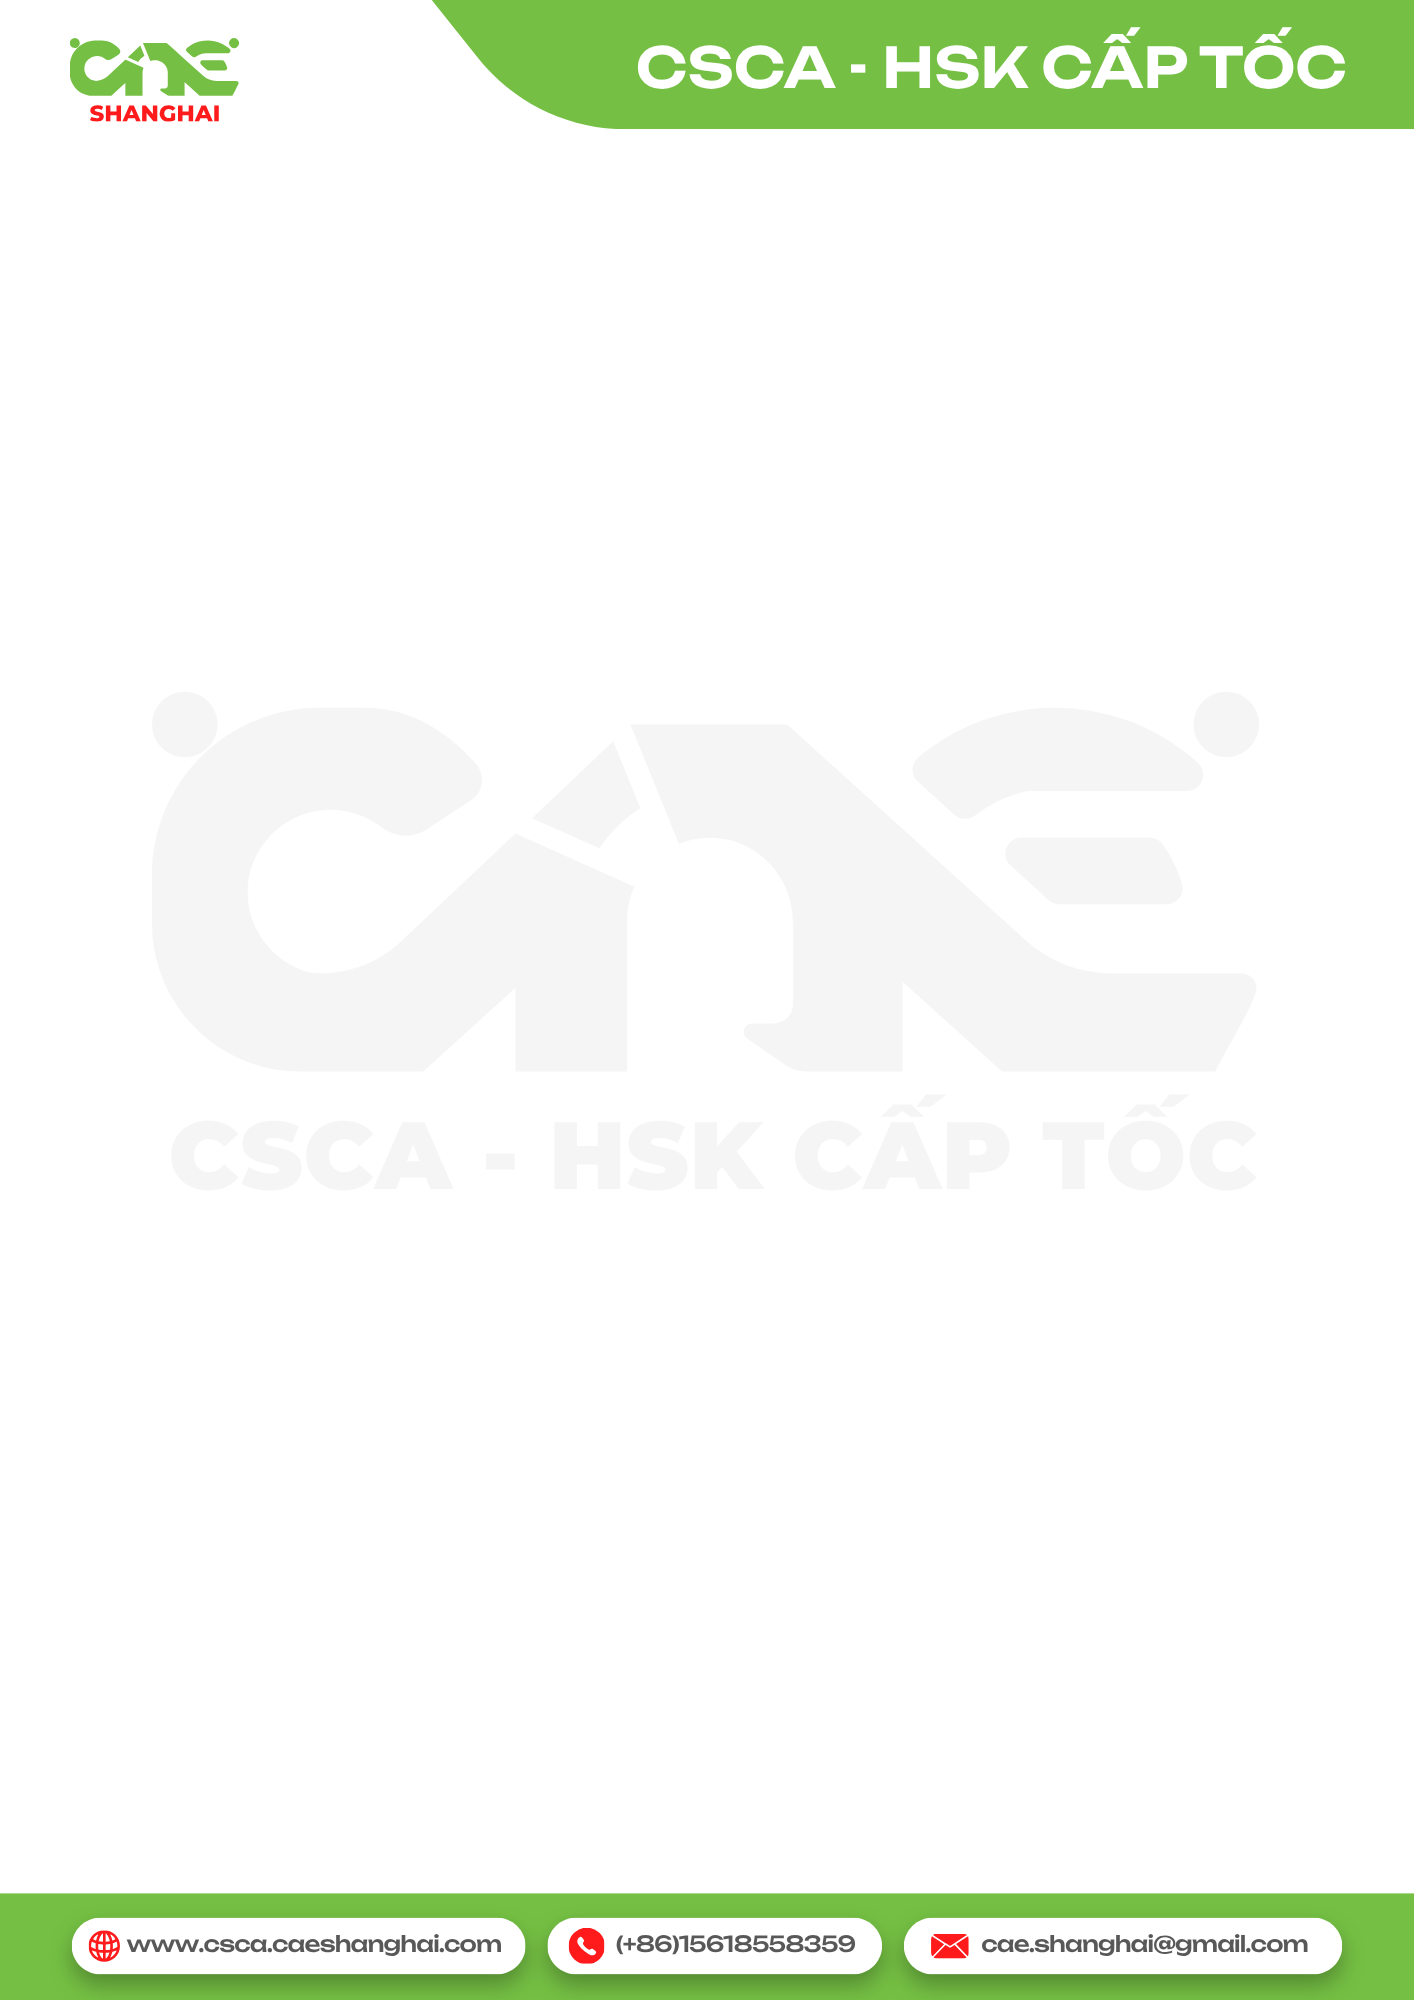
\includegraphics[width=\paperwidth,height=\paperheight]{images/letterhead.png}%
  }%
}

% ---------- ĐẦU / CHÂN TRANG ----------
% Letterhead đã có banner trên và dưới, nên bỏ dòng chạy để tránh chồng chữ.
% Số trang đặt trong vùng nội dung, sát trên banner dưới, lề phải.
\pagestyle{fancy}
\setlength{\headheight}{0pt}
\fancyhf{}
\renewcommand{\headrulewidth}{0pt}
\renewcommand{\footrulewidth}{0pt}
\fancyfoot[R]{\raisebox{0.9cm}{\small\color{cae_blue}\thepage}}

% ---------- MÔI TRƯỜNG NỘI DUNG ----------
% Trong tcolorbox, LaTeX đặt parindent = parskip = 0, nên các đoạn văn trong
% khung dính liền nhau. Đặt lại khoảng cách đoạn cho mọi khung.
\newcommand{\khoangcachdoan}{\setlength{\parskip}{0.5em}\setlength{\parindent}{0pt}}
\tcbset{before upper={\khoangcachdoan}}

\newtcolorbox{dinhnghia}[1][]{
  colback=box_bg, colframe=box_line, boxrule=0.6pt, arc=1pt,
  fonttitle=\bfseries, title={Định nghĩa #1}, breakable}
\newtcolorbox{dinhly}[1][]{
  colback=box_bg, colframe=cae_gold, boxrule=0.6pt, arc=1pt,
  fonttitle=\bfseries, title={Tính chất #1}, breakable}
\newtcolorbox{vidu}[1][]{
  colback=white, colframe=black!40, boxrule=0.4pt, arc=1pt,
  fonttitle=\bfseries, title={Ví dụ #1}, breakable}
\newtcolorbox{baitap}[1][]{
  colback=white, colframe=cae_blue!50, boxrule=0.4pt, arc=1pt,
  fonttitle=\bfseries, title={Câu #1}, breakable}

% Ô đáp án: viền xanh đậm hơn, dùng trong file đáp án
\newtcolorbox{dapan}[1][]{
  colback=box_bg, colframe=cae_blue, boxrule=0.6pt, arc=1pt,
  fonttitle=\bfseries, title={Câu #1}, breakable}

% ---------- TÊN CHỨNG MINH ----------
\renewcommand{\proofname}{\normalfont\bfseries Chứng minh}

% ---------- MÔN HỌC ----------
% Đổi được ở file .tex trước khi % =====================================================================
%  CAE SHANGHAI — GÓI LỆNH DÙNG CHUNG CHO TÀI LIỆU LUYỆN THI CSCA TOÁN
%  Biên dịch bằng XeLaTeX. Mọi file .tex trong buổi học \input file này.
% =====================================================================

% ---------- NGÔN NGỮ & PHÔNG CHỮ ----------
\usepackage{fontspec}
\usepackage{polyglossia}
\setmainlanguage{vietnamese}
\setotherlanguage{english}

% Chữ Latin (Anh + Việt): TeX Gyre Termes — bản clone Times New Roman,
% đi kèm TeX Live, hỗ trợ đầy đủ dấu tiếng Việt.
\setmainfont{TeX Gyre Termes}
\setsansfont{TeX Gyre Heros}

% Chữ Hán: ưu tiên Source Han Serif SC (思源宋体) — chuẩn học thuật Trung Quốc.
% Nếu máy chưa cài, tự động dùng Songti SC (宋体, có sẵn trên macOS).
% Cả hai đều thuộc họ 宋体 nên diện mạo tài liệu không đổi.
\IfFontExistsTF{Source Han Serif SC}{
  \newcommand{\cjkfamilyname}{Source Han Serif SC}
}{
  \IfFontExistsTF{Songti SC}{
    \newcommand{\cjkfamilyname}{Songti SC}
  }{
    \newcommand{\cjkfamilyname}{Noto Serif CJK SC}
  }
}

% xeCJK tự chuyển font khi gặp ký tự Hán, không cần bọc \cjk{} thủ công.
% Đây là điều kiện bắt buộc: font Latin (TeX Gyre Termes) không có glyph chữ Hán,
% nếu không khai báo xeCJK thì mọi chữ Hán viết trần sẽ bị nuốt khỏi bản in.
\usepackage{xeCJK}
\setCJKfamilyfont{caehan}{\cjkfamilyname}[Scale=0.95]
\setCJKmainfont{\cjkfamilyname}[Scale=0.95]
\setCJKsansfont{\cjkfamilyname}[Scale=0.95]
\setCJKmonofont{\cjkfamilyname}[Scale=0.95]

% \cjk{} ép dùng font Hán trong ngữ cảnh cần thiết (ví dụ trong tiêu đề in đậm
% hoặc trong bảng có định dạng riêng). Dùng \CJKfamily chứ không phải tên font,
% vì tên font chỉ là văn bản — sẽ in ra chữ thay vì đổi font.
\newcommand{\cjk}[1]{{\CJKfamily{caehan}#1}}

% ---------- TOÁN HỌC ----------
\usepackage{amsmath, amssymb, amsthm, mathtools}
\usepackage{unicode-math}
\setmathfont{TeX Gyre Termes Math}

% ---------- BỐ CỤC TRANG ----------
% Lề phải chừa vùng an toàn của letterhead:
%   banner trên chiếm 0–19mm  → top tối thiểu 2,2cm
%   banner dưới chiếm 281–297mm → bottom tối thiểu 2,2cm
% Lề trên 2,6cm (26mm) để tiêu đề đầu trang không đè banner (banner hết ở 19mm).
\usepackage[a4paper, top=2.6cm, bottom=2.4cm, left=2.5cm, right=2.0cm]{geometry}
\usepackage{fancyhdr}
\usepackage{titlesec}
\usepackage{enumitem}
\usepackage{graphicx}
\usepackage{booktabs, array, longtable, tabularx}
\usepackage{xcolor}
\usepackage[most]{tcolorbox}
\usepackage[colorlinks=true, linkcolor=cae_blue, citecolor=cae_blue, urlcolor=cae_blue]{hyperref}

% ---------- BẢNG MÀU THƯƠNG HIỆU ----------
\definecolor{cae_blue}{RGB}{0, 51, 102}
\definecolor{cae_gold}{RGB}{196, 149, 60}
\definecolor{box_bg}{RGB}{245, 247, 250}
\definecolor{box_line}{RGB}{0, 51, 102}

% ---------- TIÊU ĐỀ MỤC ----------
% Đệm đầu trang: banner letterhead chiếm 0–19mm, mà lề trên là 22mm.
% \section* đầu trang (sau \clearpage) sát lề nên phải chừa thêm, nếu không
% sẽ đè lên banner.
\titleformat{\section}
  {\normalfont\large\bfseries\sffamily\color{cae_blue}}{\thesection.}{0.6em}{}
\titleformat{\subsection}
  {\normalfont\normalsize\bfseries\sffamily\color{cae_blue!85!black}}{\thesubsection}{0.6em}{}
\titlespacing*{\section}{0pt}{14pt}{6pt}
\titlespacing*{\subsection}{0pt}{10pt}{4pt}

% Tiêu đề không đánh số ở đầu trang: \section* sau \clearpage nằm sát lề trên
% nên đè lên banner letterhead. Dùng \vspace* ngay TRƯỚC \section* không đủ,
% vì titlesec chèn khoảng cách riêng. Cách chắc chắn là đệm bằng \null.
\newcommand{\sectiondautrang}[1]{\section*{#1}}

% Dạng bài dùng \subsection*{} nên cần định dạng riêng, đậm và có gạch chân màu
\titleformat{\subsubsection}
  {\normalfont\normalsize\bfseries\sffamily\color{cae_blue!85!black}}{\thesubsubsection}{0.6em}{}

% ---------- LETTERHEAD (ảnh nền toàn trang) ----------
% Ảnh letterhead của CAE Shanghai: banner xanh trên/dưới kèm logo chìm giữa.
% Tỉ lệ ảnh 1414x2000 = 0.7070, khớp A4 (0.7071) nên chèn thẳng không méo.
% Đặt ở lớp nền dưới cùng để chữ không bị ảnh che.
% Dùng \AddToShipoutPictureBG (không có dấu *) để áp dụng cho MỌI trang.
\usepackage{eso-pic}
\AddToShipoutPictureBG{%
  \AtPageLowerLeft{%
    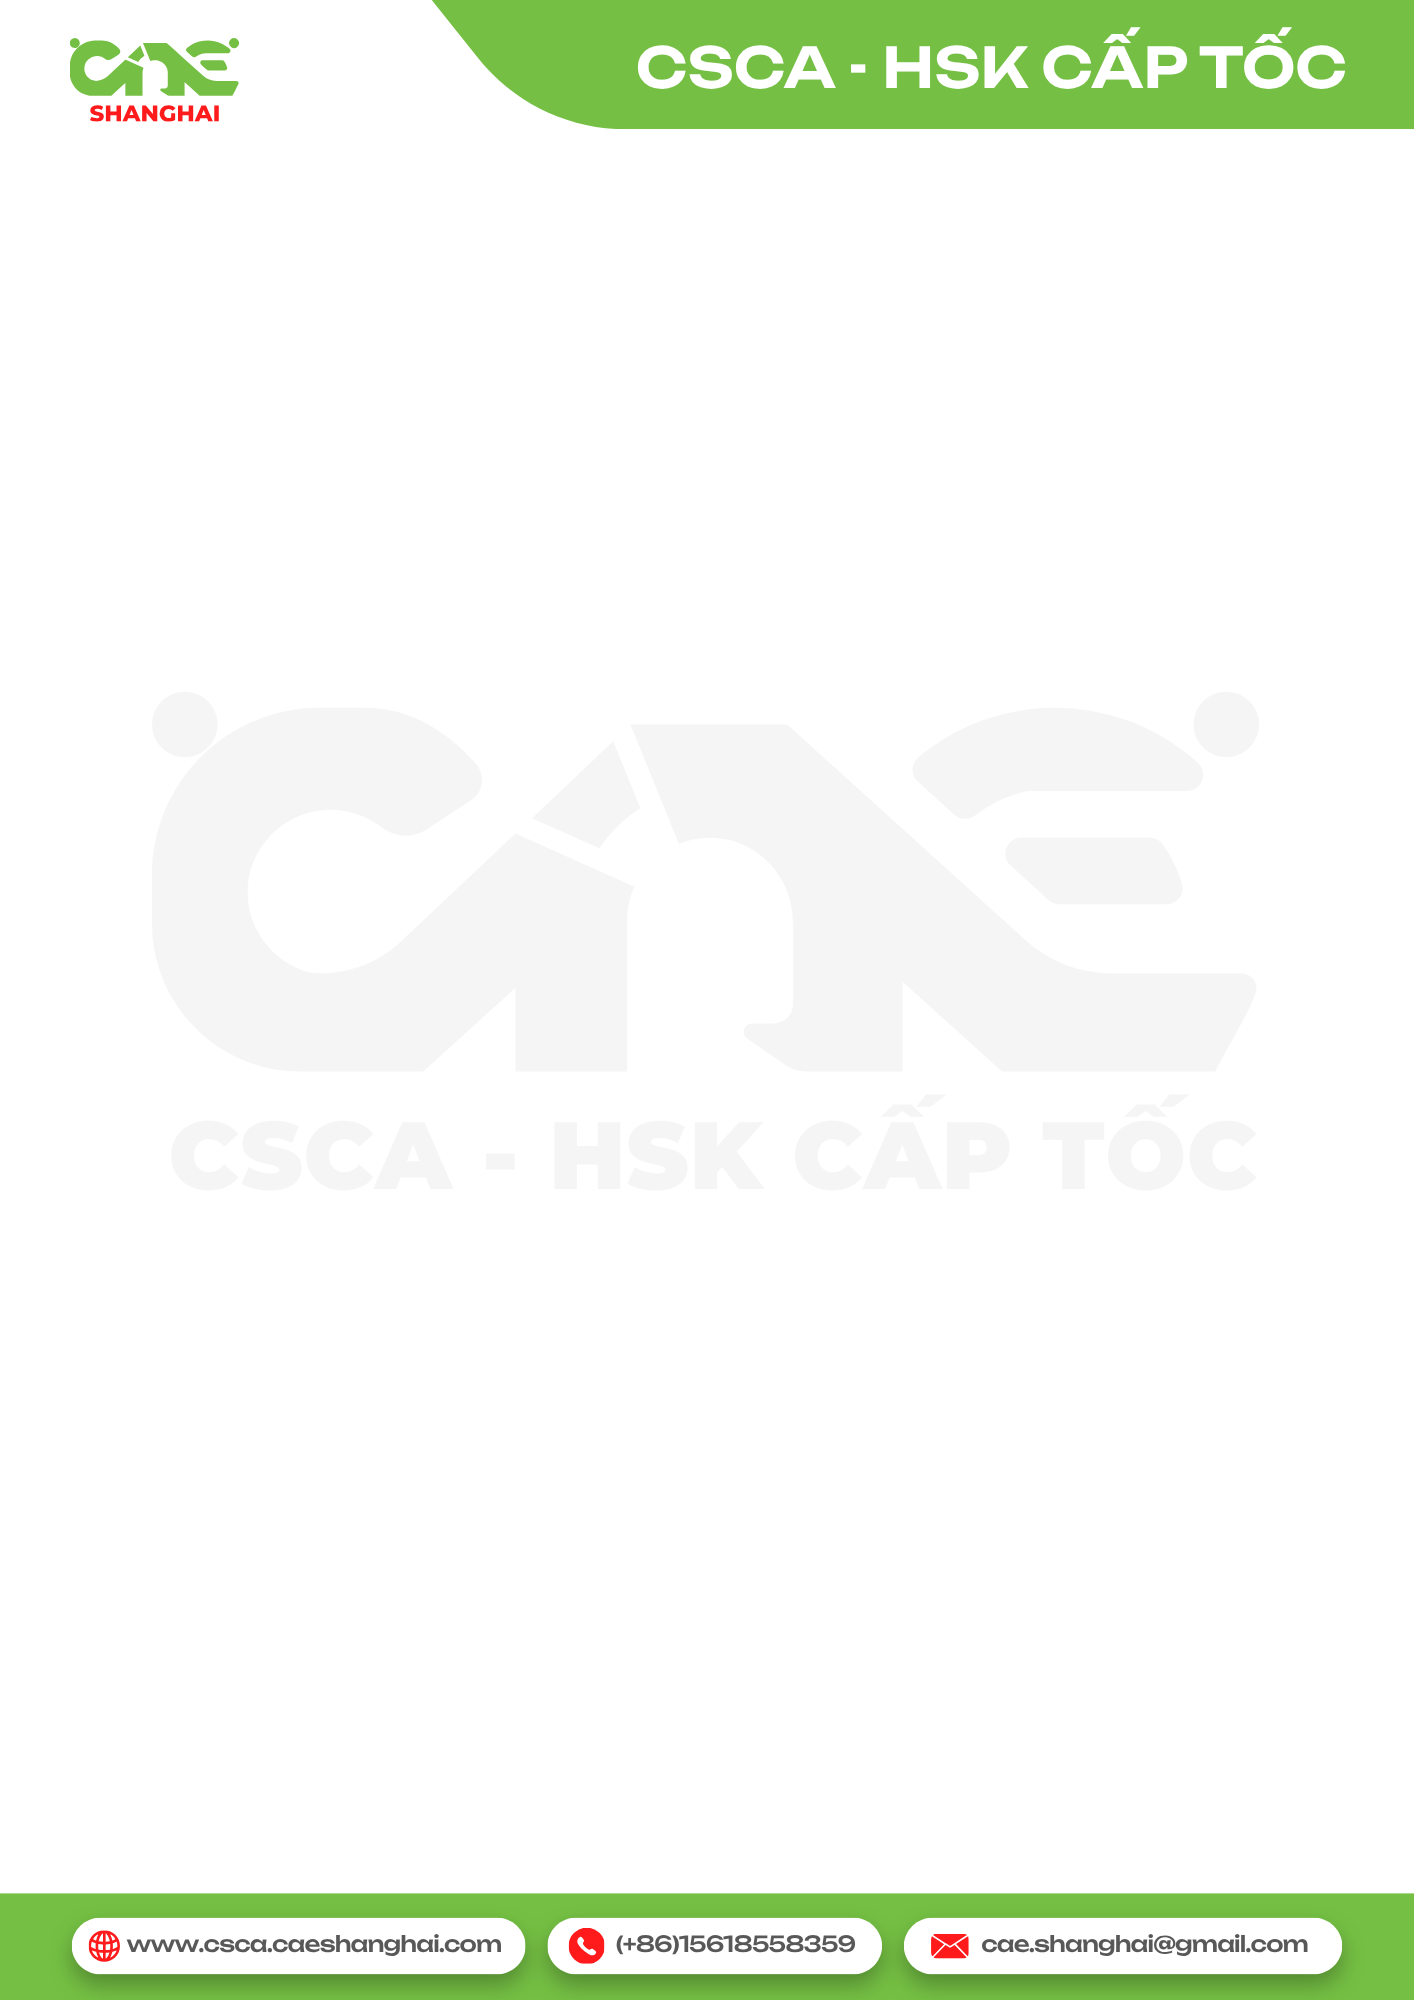
\includegraphics[width=\paperwidth,height=\paperheight]{images/letterhead.png}%
  }%
}

% ---------- ĐẦU / CHÂN TRANG ----------
% Letterhead đã có banner trên và dưới, nên bỏ dòng chạy để tránh chồng chữ.
% Số trang đặt trong vùng nội dung, sát trên banner dưới, lề phải.
\pagestyle{fancy}
\setlength{\headheight}{0pt}
\fancyhf{}
\renewcommand{\headrulewidth}{0pt}
\renewcommand{\footrulewidth}{0pt}
\fancyfoot[R]{\raisebox{0.9cm}{\small\color{cae_blue}\thepage}}

% ---------- MÔI TRƯỜNG NỘI DUNG ----------
% Trong tcolorbox, LaTeX đặt parindent = parskip = 0, nên các đoạn văn trong
% khung dính liền nhau. Đặt lại khoảng cách đoạn cho mọi khung.
\newcommand{\khoangcachdoan}{\setlength{\parskip}{0.5em}\setlength{\parindent}{0pt}}
\tcbset{before upper={\khoangcachdoan}}

\newtcolorbox{dinhnghia}[1][]{
  colback=box_bg, colframe=box_line, boxrule=0.6pt, arc=1pt,
  fonttitle=\bfseries, title={Định nghĩa #1}, breakable}
\newtcolorbox{dinhly}[1][]{
  colback=box_bg, colframe=cae_gold, boxrule=0.6pt, arc=1pt,
  fonttitle=\bfseries, title={Tính chất #1}, breakable}
\newtcolorbox{vidu}[1][]{
  colback=white, colframe=black!40, boxrule=0.4pt, arc=1pt,
  fonttitle=\bfseries, title={Ví dụ #1}, breakable}
\newtcolorbox{baitap}[1][]{
  colback=white, colframe=cae_blue!50, boxrule=0.4pt, arc=1pt,
  fonttitle=\bfseries, title={Câu #1}, breakable}

% Ô đáp án: viền xanh đậm hơn, dùng trong file đáp án
\newtcolorbox{dapan}[1][]{
  colback=box_bg, colframe=cae_blue, boxrule=0.6pt, arc=1pt,
  fonttitle=\bfseries, title={Câu #1}, breakable}

% ---------- TÊN CHỨNG MINH ----------
\renewcommand{\proofname}{\normalfont\bfseries Chứng minh}

% ---------- MÔN HỌC ----------
% Đổi được ở file .tex trước khi % =====================================================================
%  CAE SHANGHAI — GÓI LỆNH DÙNG CHUNG CHO TÀI LIỆU LUYỆN THI CSCA TOÁN
%  Biên dịch bằng XeLaTeX. Mọi file .tex trong buổi học \input file này.
% =====================================================================

% ---------- NGÔN NGỮ & PHÔNG CHỮ ----------
\usepackage{fontspec}
\usepackage{polyglossia}
\setmainlanguage{vietnamese}
\setotherlanguage{english}

% Chữ Latin (Anh + Việt): TeX Gyre Termes — bản clone Times New Roman,
% đi kèm TeX Live, hỗ trợ đầy đủ dấu tiếng Việt.
\setmainfont{TeX Gyre Termes}
\setsansfont{TeX Gyre Heros}

% Chữ Hán: ưu tiên Source Han Serif SC (思源宋体) — chuẩn học thuật Trung Quốc.
% Nếu máy chưa cài, tự động dùng Songti SC (宋体, có sẵn trên macOS).
% Cả hai đều thuộc họ 宋体 nên diện mạo tài liệu không đổi.
\IfFontExistsTF{Source Han Serif SC}{
  \newcommand{\cjkfamilyname}{Source Han Serif SC}
}{
  \IfFontExistsTF{Songti SC}{
    \newcommand{\cjkfamilyname}{Songti SC}
  }{
    \newcommand{\cjkfamilyname}{Noto Serif CJK SC}
  }
}

% xeCJK tự chuyển font khi gặp ký tự Hán, không cần bọc \cjk{} thủ công.
% Đây là điều kiện bắt buộc: font Latin (TeX Gyre Termes) không có glyph chữ Hán,
% nếu không khai báo xeCJK thì mọi chữ Hán viết trần sẽ bị nuốt khỏi bản in.
\usepackage{xeCJK}
\setCJKfamilyfont{caehan}{\cjkfamilyname}[Scale=0.95]
\setCJKmainfont{\cjkfamilyname}[Scale=0.95]
\setCJKsansfont{\cjkfamilyname}[Scale=0.95]
\setCJKmonofont{\cjkfamilyname}[Scale=0.95]

% \cjk{} ép dùng font Hán trong ngữ cảnh cần thiết (ví dụ trong tiêu đề in đậm
% hoặc trong bảng có định dạng riêng). Dùng \CJKfamily chứ không phải tên font,
% vì tên font chỉ là văn bản — sẽ in ra chữ thay vì đổi font.
\newcommand{\cjk}[1]{{\CJKfamily{caehan}#1}}

% ---------- TOÁN HỌC ----------
\usepackage{amsmath, amssymb, amsthm, mathtools}
\usepackage{unicode-math}
\setmathfont{TeX Gyre Termes Math}

% ---------- BỐ CỤC TRANG ----------
% Lề phải chừa vùng an toàn của letterhead:
%   banner trên chiếm 0–19mm  → top tối thiểu 2,2cm
%   banner dưới chiếm 281–297mm → bottom tối thiểu 2,2cm
% Lề trên 2,6cm (26mm) để tiêu đề đầu trang không đè banner (banner hết ở 19mm).
\usepackage[a4paper, top=2.6cm, bottom=2.4cm, left=2.5cm, right=2.0cm]{geometry}
\usepackage{fancyhdr}
\usepackage{titlesec}
\usepackage{enumitem}
\usepackage{graphicx}
\usepackage{booktabs, array, longtable, tabularx}
\usepackage{xcolor}
\usepackage[most]{tcolorbox}
\usepackage[colorlinks=true, linkcolor=cae_blue, citecolor=cae_blue, urlcolor=cae_blue]{hyperref}

% ---------- BẢNG MÀU THƯƠNG HIỆU ----------
\definecolor{cae_blue}{RGB}{0, 51, 102}
\definecolor{cae_gold}{RGB}{196, 149, 60}
\definecolor{box_bg}{RGB}{245, 247, 250}
\definecolor{box_line}{RGB}{0, 51, 102}

% ---------- TIÊU ĐỀ MỤC ----------
% Đệm đầu trang: banner letterhead chiếm 0–19mm, mà lề trên là 22mm.
% \section* đầu trang (sau \clearpage) sát lề nên phải chừa thêm, nếu không
% sẽ đè lên banner.
\titleformat{\section}
  {\normalfont\large\bfseries\sffamily\color{cae_blue}}{\thesection.}{0.6em}{}
\titleformat{\subsection}
  {\normalfont\normalsize\bfseries\sffamily\color{cae_blue!85!black}}{\thesubsection}{0.6em}{}
\titlespacing*{\section}{0pt}{14pt}{6pt}
\titlespacing*{\subsection}{0pt}{10pt}{4pt}

% Tiêu đề không đánh số ở đầu trang: \section* sau \clearpage nằm sát lề trên
% nên đè lên banner letterhead. Dùng \vspace* ngay TRƯỚC \section* không đủ,
% vì titlesec chèn khoảng cách riêng. Cách chắc chắn là đệm bằng \null.
\newcommand{\sectiondautrang}[1]{\section*{#1}}

% Dạng bài dùng \subsection*{} nên cần định dạng riêng, đậm và có gạch chân màu
\titleformat{\subsubsection}
  {\normalfont\normalsize\bfseries\sffamily\color{cae_blue!85!black}}{\thesubsubsection}{0.6em}{}

% ---------- LETTERHEAD (ảnh nền toàn trang) ----------
% Ảnh letterhead của CAE Shanghai: banner xanh trên/dưới kèm logo chìm giữa.
% Tỉ lệ ảnh 1414x2000 = 0.7070, khớp A4 (0.7071) nên chèn thẳng không méo.
% Đặt ở lớp nền dưới cùng để chữ không bị ảnh che.
% Dùng \AddToShipoutPictureBG (không có dấu *) để áp dụng cho MỌI trang.
\usepackage{eso-pic}
\AddToShipoutPictureBG{%
  \AtPageLowerLeft{%
    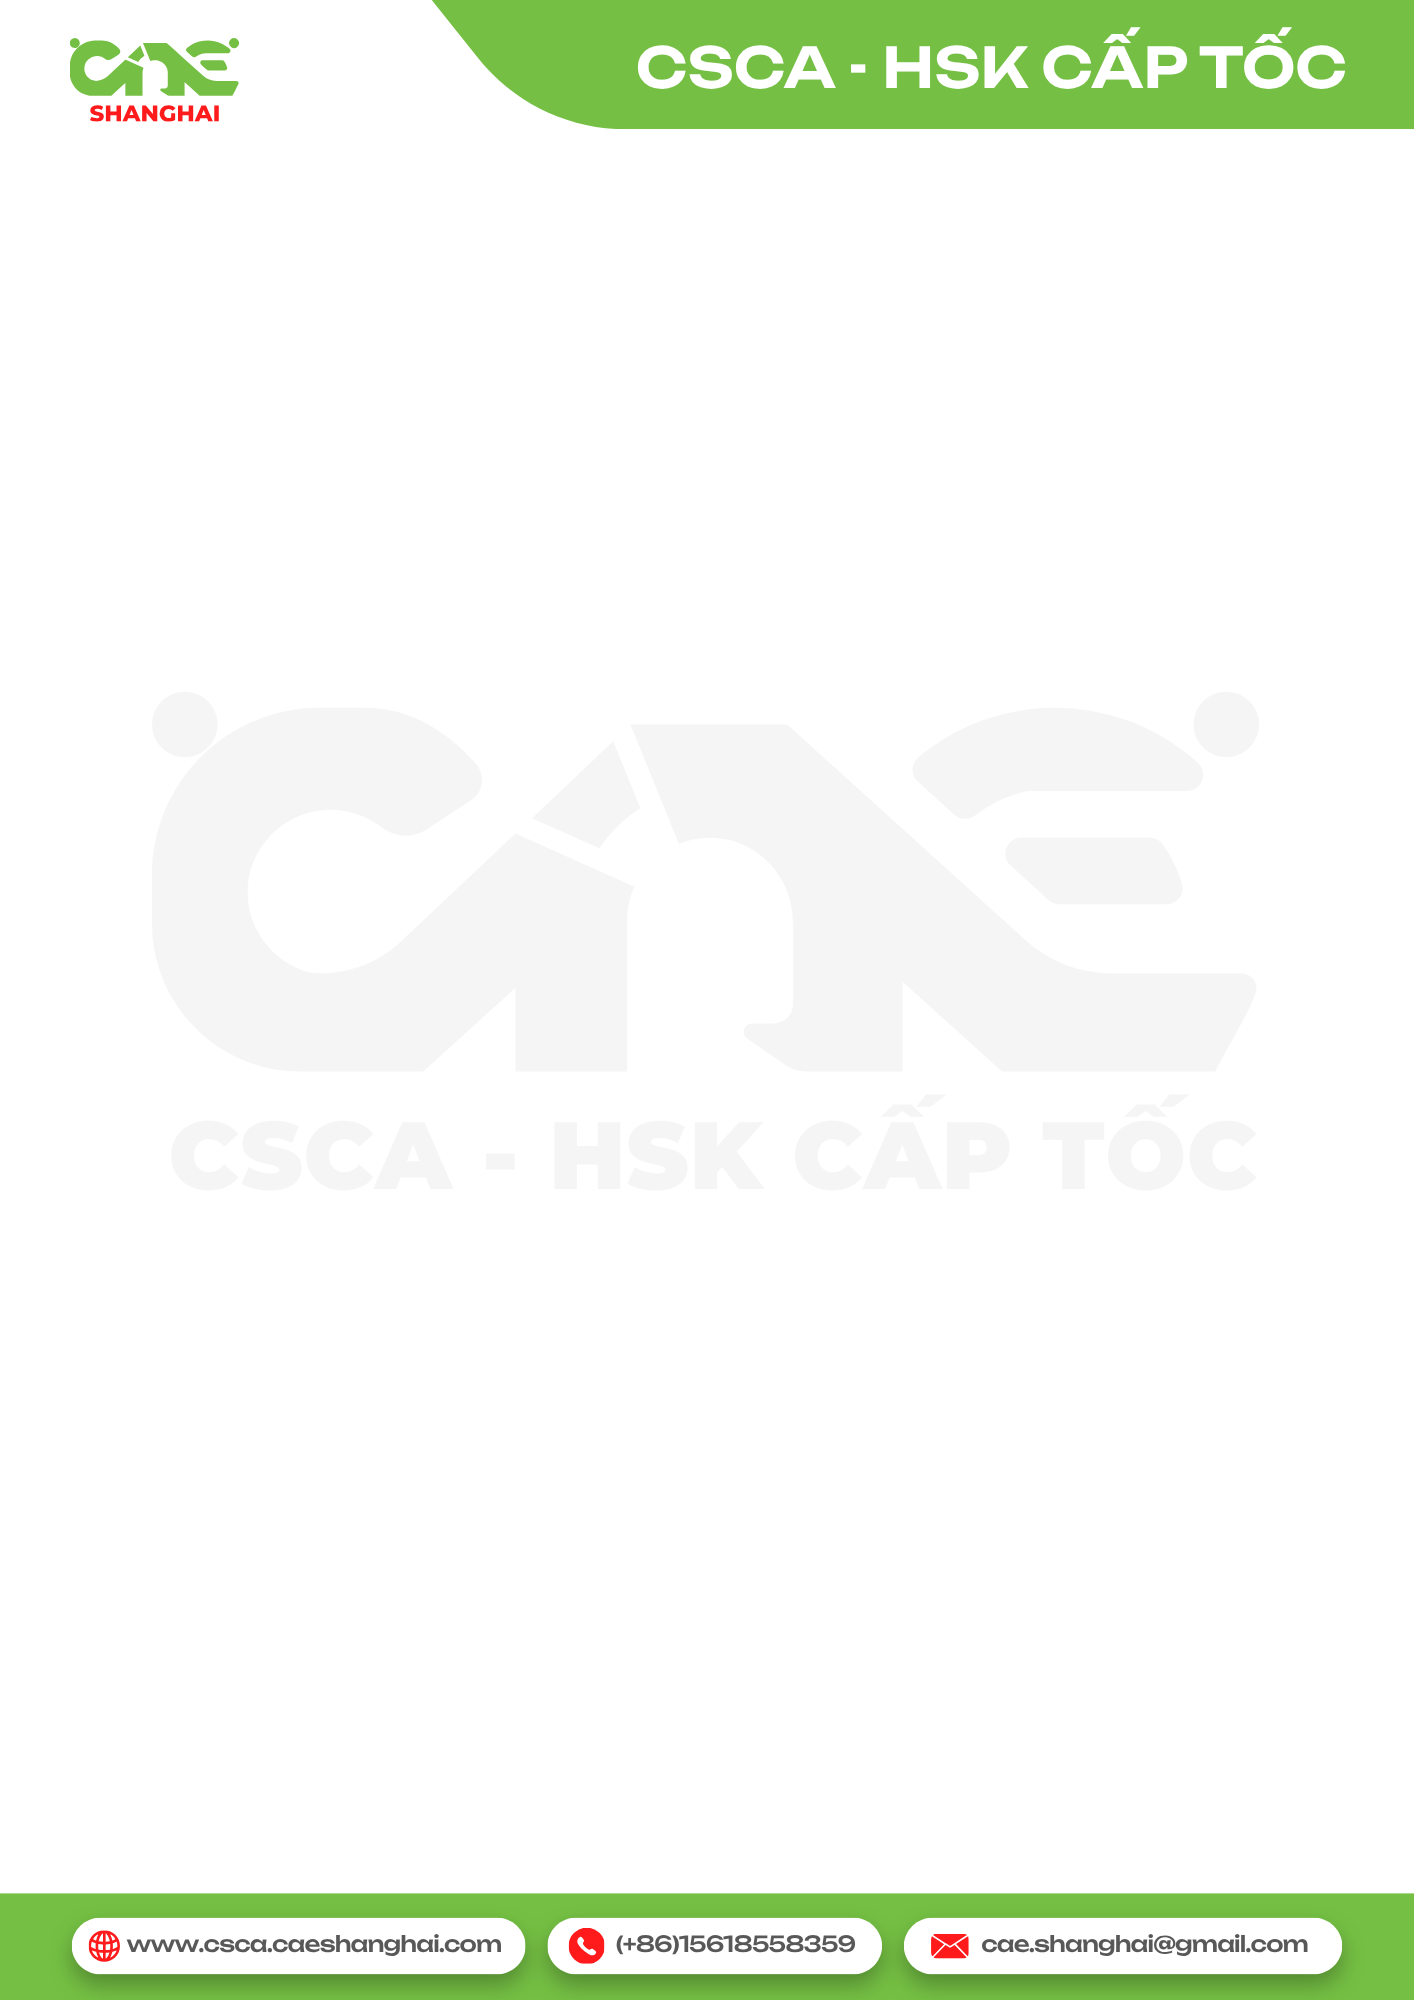
\includegraphics[width=\paperwidth,height=\paperheight]{images/letterhead.png}%
  }%
}

% ---------- ĐẦU / CHÂN TRANG ----------
% Letterhead đã có banner trên và dưới, nên bỏ dòng chạy để tránh chồng chữ.
% Số trang đặt trong vùng nội dung, sát trên banner dưới, lề phải.
\pagestyle{fancy}
\setlength{\headheight}{0pt}
\fancyhf{}
\renewcommand{\headrulewidth}{0pt}
\renewcommand{\footrulewidth}{0pt}
\fancyfoot[R]{\raisebox{0.9cm}{\small\color{cae_blue}\thepage}}

% ---------- MÔI TRƯỜNG NỘI DUNG ----------
% Trong tcolorbox, LaTeX đặt parindent = parskip = 0, nên các đoạn văn trong
% khung dính liền nhau. Đặt lại khoảng cách đoạn cho mọi khung.
\newcommand{\khoangcachdoan}{\setlength{\parskip}{0.5em}\setlength{\parindent}{0pt}}
\tcbset{before upper={\khoangcachdoan}}

\newtcolorbox{dinhnghia}[1][]{
  colback=box_bg, colframe=box_line, boxrule=0.6pt, arc=1pt,
  fonttitle=\bfseries, title={Định nghĩa #1}, breakable}
\newtcolorbox{dinhly}[1][]{
  colback=box_bg, colframe=cae_gold, boxrule=0.6pt, arc=1pt,
  fonttitle=\bfseries, title={Tính chất #1}, breakable}
\newtcolorbox{vidu}[1][]{
  colback=white, colframe=black!40, boxrule=0.4pt, arc=1pt,
  fonttitle=\bfseries, title={Ví dụ #1}, breakable}
\newtcolorbox{baitap}[1][]{
  colback=white, colframe=cae_blue!50, boxrule=0.4pt, arc=1pt,
  fonttitle=\bfseries, title={Câu #1}, breakable}

% Ô đáp án: viền xanh đậm hơn, dùng trong file đáp án
\newtcolorbox{dapan}[1][]{
  colback=box_bg, colframe=cae_blue, boxrule=0.6pt, arc=1pt,
  fonttitle=\bfseries, title={Câu #1}, breakable}

% ---------- TÊN CHỨNG MINH ----------
\renewcommand{\proofname}{\normalfont\bfseries Chứng minh}

% ---------- MÔN HỌC ----------
% Đổi được ở file .tex trước khi \input{cae-style} bằng \renewcommand{\monhoc}{...}
\providecommand{\monhoc}{Môn Toán}

% ---------- TRANG BÌA GỌN ----------
% #1 = loại tài liệu (TÀI LIỆU CHUẨN BỊ, TÀI LIỆU BUỔI HỌC, ...)
% #2 = số buổi
% #3 = tên buổi tiếng Việt
% #4 = tên buổi tiếng Hán
% #5 = module và tỉ trọng
\newcommand{\trangbia}[5]{%
  \begin{center}
    \vspace*{0.6cm}
    {\large\bfseries\color{cae_blue} CAE SHANGHAI}\\[0.15cm]
    {\footnotesize Tài liệu luyện thi CSCA · \monhoc}\\[0.5cm]
    {\color{cae_gold}\rule{0.55\linewidth}{0.8pt}}\\[0.35cm]
    {\small\bfseries\color{cae_blue!80!black} #1}\\[0.35cm]
    {\Large\bfseries\color{cae_blue} BUỔI #2 — #3}\\[0.2cm]
    {\large\color{cae_blue!85!black} \cjk{#4}}\\[0.25cm]
    \ifx\relax#5\relax\else{\small #5}\\[0.35cm]\fi
    {\color{cae_gold}\rule{0.55\linewidth}{0.8pt}}\\[0.3cm]
    {\footnotesize Biên soạn: Hoàng Dương, CAE Shanghai \quad·\quad \today}
  \end{center}
  \vspace{0.3cm}
}

% ---------- TRANG BÌA CHO ĐỀ KIỂM TRA ----------
% Khác \trangbia ở chỗ không có chữ "BUỔI N" — dùng cho đề thi, không phải bài giảng.
% #1 = loại tài liệu, #2 = tên kỳ thi (Việt), #3 = tên kỳ thi (Hán), #4 = thông số
\newcommand{\biade}[4]{%
  \begin{center}
    \vspace*{0.6cm}
    {\large\bfseries\color{cae_blue} CAE SHANGHAI}\\[0.15cm]
    {\footnotesize Tài liệu luyện thi CSCA · \monhoc}\\[0.5cm]
    {\color{cae_gold}\rule{0.55\linewidth}{0.8pt}}\\[0.35cm]
    {\small\bfseries\color{cae_blue!80!black} #1}\\[0.35cm]
    {\Large\bfseries\color{cae_blue} #2}\\[0.2cm]
    {\large\color{cae_blue!85!black} \cjk{#3}}\\[0.25cm]
    {\small #4}\\[0.35cm]
    {\color{cae_gold}\rule{0.55\linewidth}{0.8pt}}\\[0.3cm]
    {\footnotesize Biên soạn: Hoàng Dương, CAE Shanghai \quad·\quad \today}
  \end{center}
  \vspace{0.3cm}
}

% ---------- TIỆN ÍCH ----------
% Nhãn từ khóa in đậm ở đầu đoạn, dùng cho Từ vựng / Từ khóa nhận dạng / Chú ý
% Khoảng cách đoạn do khung tự đặt (xem \khoangcachdoan ở trên),
% ở đây chỉ cần tách đoạn và bỏ thụt đầu dòng.
\newcommand{\nhan}[1]{\par\noindent\textbf{#1.}\ \ignorespaces}

% Bảng gọn, không đánh số
\newcommand{\bang}[1]{%
  \begin{center}#1\end{center}}

% Đánh dấu ô trống cho học sinh điền
\newcommand{\chotrong}{\makebox[3.2cm]{\dotfill}}
 bằng \renewcommand{\monhoc}{...}
\providecommand{\monhoc}{Môn Toán}

% ---------- TRANG BÌA GỌN ----------
% #1 = loại tài liệu (TÀI LIỆU CHUẨN BỊ, TÀI LIỆU BUỔI HỌC, ...)
% #2 = số buổi
% #3 = tên buổi tiếng Việt
% #4 = tên buổi tiếng Hán
% #5 = module và tỉ trọng
\newcommand{\trangbia}[5]{%
  \begin{center}
    \vspace*{0.6cm}
    {\large\bfseries\color{cae_blue} CAE SHANGHAI}\\[0.15cm]
    {\footnotesize Tài liệu luyện thi CSCA · \monhoc}\\[0.5cm]
    {\color{cae_gold}\rule{0.55\linewidth}{0.8pt}}\\[0.35cm]
    {\small\bfseries\color{cae_blue!80!black} #1}\\[0.35cm]
    {\Large\bfseries\color{cae_blue} BUỔI #2 — #3}\\[0.2cm]
    {\large\color{cae_blue!85!black} \cjk{#4}}\\[0.25cm]
    \ifx\relax#5\relax\else{\small #5}\\[0.35cm]\fi
    {\color{cae_gold}\rule{0.55\linewidth}{0.8pt}}\\[0.3cm]
    {\footnotesize Biên soạn: Hoàng Dương, CAE Shanghai \quad·\quad \today}
  \end{center}
  \vspace{0.3cm}
}

% ---------- TRANG BÌA CHO ĐỀ KIỂM TRA ----------
% Khác \trangbia ở chỗ không có chữ "BUỔI N" — dùng cho đề thi, không phải bài giảng.
% #1 = loại tài liệu, #2 = tên kỳ thi (Việt), #3 = tên kỳ thi (Hán), #4 = thông số
\newcommand{\biade}[4]{%
  \begin{center}
    \vspace*{0.6cm}
    {\large\bfseries\color{cae_blue} CAE SHANGHAI}\\[0.15cm]
    {\footnotesize Tài liệu luyện thi CSCA · \monhoc}\\[0.5cm]
    {\color{cae_gold}\rule{0.55\linewidth}{0.8pt}}\\[0.35cm]
    {\small\bfseries\color{cae_blue!80!black} #1}\\[0.35cm]
    {\Large\bfseries\color{cae_blue} #2}\\[0.2cm]
    {\large\color{cae_blue!85!black} \cjk{#3}}\\[0.25cm]
    {\small #4}\\[0.35cm]
    {\color{cae_gold}\rule{0.55\linewidth}{0.8pt}}\\[0.3cm]
    {\footnotesize Biên soạn: Hoàng Dương, CAE Shanghai \quad·\quad \today}
  \end{center}
  \vspace{0.3cm}
}

% ---------- TIỆN ÍCH ----------
% Nhãn từ khóa in đậm ở đầu đoạn, dùng cho Từ vựng / Từ khóa nhận dạng / Chú ý
% Khoảng cách đoạn do khung tự đặt (xem \khoangcachdoan ở trên),
% ở đây chỉ cần tách đoạn và bỏ thụt đầu dòng.
\newcommand{\nhan}[1]{\par\noindent\textbf{#1.}\ \ignorespaces}

% Bảng gọn, không đánh số
\newcommand{\bang}[1]{%
  \begin{center}#1\end{center}}

% Đánh dấu ô trống cho học sinh điền
\newcommand{\chotrong}{\makebox[3.2cm]{\dotfill}}
 bằng \renewcommand{\monhoc}{...}
\providecommand{\monhoc}{Môn Toán}

% ---------- TRANG BÌA GỌN ----------
% #1 = loại tài liệu (TÀI LIỆU CHUẨN BỊ, TÀI LIỆU BUỔI HỌC, ...)
% #2 = số buổi
% #3 = tên buổi tiếng Việt
% #4 = tên buổi tiếng Hán
% #5 = module và tỉ trọng
\newcommand{\trangbia}[5]{%
  \begin{center}
    \vspace*{0.6cm}
    {\large\bfseries\color{cae_blue} CAE SHANGHAI}\\[0.15cm]
    {\footnotesize Tài liệu luyện thi CSCA · \monhoc}\\[0.5cm]
    {\color{cae_gold}\rule{0.55\linewidth}{0.8pt}}\\[0.35cm]
    {\small\bfseries\color{cae_blue!80!black} #1}\\[0.35cm]
    {\Large\bfseries\color{cae_blue} BUỔI #2 — #3}\\[0.2cm]
    {\large\color{cae_blue!85!black} \cjk{#4}}\\[0.25cm]
    \ifx\relax#5\relax\else{\small #5}\\[0.35cm]\fi
    {\color{cae_gold}\rule{0.55\linewidth}{0.8pt}}\\[0.3cm]
    {\footnotesize Biên soạn: Hoàng Dương, CAE Shanghai \quad·\quad \today}
  \end{center}
  \vspace{0.3cm}
}

% ---------- TRANG BÌA CHO ĐỀ KIỂM TRA ----------
% Khác \trangbia ở chỗ không có chữ "BUỔI N" — dùng cho đề thi, không phải bài giảng.
% #1 = loại tài liệu, #2 = tên kỳ thi (Việt), #3 = tên kỳ thi (Hán), #4 = thông số
\newcommand{\biade}[4]{%
  \begin{center}
    \vspace*{0.6cm}
    {\large\bfseries\color{cae_blue} CAE SHANGHAI}\\[0.15cm]
    {\footnotesize Tài liệu luyện thi CSCA · \monhoc}\\[0.5cm]
    {\color{cae_gold}\rule{0.55\linewidth}{0.8pt}}\\[0.35cm]
    {\small\bfseries\color{cae_blue!80!black} #1}\\[0.35cm]
    {\Large\bfseries\color{cae_blue} #2}\\[0.2cm]
    {\large\color{cae_blue!85!black} \cjk{#3}}\\[0.25cm]
    {\small #4}\\[0.35cm]
    {\color{cae_gold}\rule{0.55\linewidth}{0.8pt}}\\[0.3cm]
    {\footnotesize Biên soạn: Hoàng Dương, CAE Shanghai \quad·\quad \today}
  \end{center}
  \vspace{0.3cm}
}

% ---------- TIỆN ÍCH ----------
% Nhãn từ khóa in đậm ở đầu đoạn, dùng cho Từ vựng / Từ khóa nhận dạng / Chú ý
% Khoảng cách đoạn do khung tự đặt (xem \khoangcachdoan ở trên),
% ở đây chỉ cần tách đoạn và bỏ thụt đầu dòng.
\newcommand{\nhan}[1]{\par\noindent\textbf{#1.}\ \ignorespaces}

% Bảng gọn, không đánh số
\newcommand{\bang}[1]{%
  \begin{center}#1\end{center}}

% Đánh dấu ô trống cho học sinh điền
\newcommand{\chotrong}{\makebox[3.2cm]{\dotfill}}


\begin{document}

\trangbia{TÀI LIỆU BUỔI HỌC}{9}{ĐƯỜNG THẲNG VÀ ĐƯỜNG TRÒN}{直线与圆}{Module M3 \quad·\quad Tỉ trọng đề thi $\sim$19\% (cùng hình học phẳng) \quad·\quad khoảng 8–10 câu}

\section{TỪ KHÓA NHẬN DẠNG ĐỀ}

Đọc được từ khóa là xác định được dạng bài mà không cần dịch cả đề. Bảng dưới đây gom những từ khóa quyết định của chuyên đề này.

\bang{
\begin{tabularx}{\linewidth}{@{}llX@{}}
\toprule
\textbf{Từ khóa} & \textbf{Nghĩa} & \textbf{Dạng bài tương ứng} \\
\midrule
斜率 & hệ số góc & Đọc hệ số góc từ phương trình, hoặc tìm hệ số góc qua hai điểm \\
倾斜角 & góc nghiêng & Đổi hệ số góc sang góc, chú ý khoảng $[0^\circ, 180^\circ)$ \\
截距 & khoảng chắn trên trục & Cho $y = 0$ tìm chắn trên trục hoành, cho $x = 0$ tìm chắn trên trục tung \\
平行 & song song & Hai đường thẳng cùng hệ số góc và khác khoảng chắn \\
垂直 & vuông góc & Tích hai hệ số góc bằng $-1$ \\
重合 & trùng nhau & Cùng hệ số góc và cùng khoảng chắn \\
交点 & giao điểm & Giải hệ hai phương trình đường thẳng \\
垂直平分线 & đường trung trực & Qua trung điểm và vuông góc với đoạn thẳng \\
点到直线的距离 & khoảng cách từ điểm đến đường thẳng & Thay tọa độ vào công thức khoảng cách \\
圆心 & tâm đường tròn & Đọc tâm từ dạng chính tắc hoặc lấy nửa hệ số đổi dấu \\
半径 & bán kính & Khai căn từ vế phải, hoặc dùng công thức tổng quát \\
标准方程 & phương trình chính tắc & Dạng $(x-a)^2 + (y-b)^2 = r^2$ \\
一般方程 & phương trình tổng quát & Dạng $x^2 + y^2 + Dx + Ey + F = 0$ \\
相切 & tiếp xúc & Khoảng cách từ tâm đến đường thẳng bằng bán kính \\
弦长 & độ dài dây cung & Dùng định lý Pythagoras với khoảng cách từ tâm \\
\bottomrule
\end{tabularx}}

\nhan{Chú ý} Hai từ khóa 斜率 (hệ số góc) và 倾斜角 (góc nghiêng) liên hệ qua công thức $k = \tan\alpha$ nhưng khác nhau về khoảng giá trị. Đề cho góc nghiêng thì đổi sang hệ số góc mới viết được phương trình; đề cho hệ số góc thì đổi sang góc bằng cách tra bảng góc đặc biệt. Đọc nhầm hai từ này là mất điểm chắc chắn.

\section{KIẾN THỨC TRỌNG TÂM}

\subsection{Hệ số góc và góc nghiêng}

\begin{dinhnghia}[{1 — Hệ số góc}]
Cho đường thẳng đi qua hai điểm $P_1(x_1, y_1)$ và $P_2(x_2, y_2)$ với $x_1 \ne x_2$. Hệ số góc của đường thẳng là

$$k = \frac{y_2 - y_1}{x_2 - x_1}$$
\end{dinhnghia}
\begin{dinhnghia}[{2 — Góc nghiêng}]
Góc nghiêng của đường thẳng là góc $\alpha$ tạo bởi chiều dương trục hoành và đường thẳng, đo ngược chiều kim đồng hồ, với $0^\circ \le \alpha < 180^\circ$.
\end{dinhnghia}
\begin{dinhly}[{1 — Liên hệ giữa hệ số góc và góc nghiêng}]
$$k = \tan\alpha$$

\bang{
\begin{tabularx}{\linewidth}{@{}lcX@{}}
\toprule
\textbf{Hệ số góc} & \textbf{Góc nghiêng} & \textbf{Hướng của đường thẳng} \\
\midrule
$k > 0$ & $0^\circ < \alpha < 90^\circ$ & Đi lên từ trái sang phải \\
$k = 0$ & $\alpha = 0^\circ$ & Nằm ngang \\
$k < 0$ & $90^\circ < \alpha < 180^\circ$ & Đi xuống từ trái sang phải \\
Không tồn tại & $\alpha = 90^\circ$ & Thẳng đứng \\
\bottomrule
\end{tabularx}}

\nhan{Chú ý} Đường thẳng thẳng đứng có phương trình dạng $x = c$ và \textbf{không có hệ số góc}. Gặp dạng này thì không được viết $y = kx + b$, phải giữ nguyên dạng $x = c$.

\nhan{Cách nhanh} Bốn góc nghiêng hay gặp trong đề: $k = \dfrac{\sqrt{3}}{3}$ cho $\alpha = 30^\circ$; $k = 1$ cho $\alpha = 45^\circ$; $k = \sqrt{3}$ cho $\alpha = 60^\circ$; $k = -1$ cho $\alpha = 135^\circ$. Nhớ bảng này thì đổi góc trong vài giây.
\end{dinhly}
\subsection{Các dạng phương trình đường thẳng}

\begin{dinhnghia}[{3 — Năm dạng phương trình đường thẳng}]
Cho đường thẳng đi qua điểm $(x_0, y_0)$ với hệ số góc $k$, chắn trên trục hoành là $a$ và chắn trên trục tung là $b$.

\bang{
\begin{tabularx}{\linewidth}{@{}llX@{}}
\toprule
\textbf{Dạng} & \textbf{Phương trình} & \textbf{Dùng khi} \\
\midrule
Điểm chắn góc & $y - y_0 = k(x - x_0)$ & Biết một điểm và hệ số góc \\
Chắn góc & $y = kx + b$ & Biết hệ số góc và khoảng chắn trên trục tung \\
Hai điểm & $\dfrac{y - y_1}{y_2 - y_1} = \dfrac{x - x_1}{x_2 - x_1}$ & Biết hai điểm phân biệt \\
Đoạn chắn & $\dfrac{x}{a} + \dfrac{y}{b} = 1$ & Biết cả hai khoảng chắn, với $ab \ne 0$ \\
Tổng quát & $Ax + By + C = 0$ & Dạng chuẩn của mọi đường thẳng \\
\bottomrule
\end{tabularx}}

\nhan{Chú ý} Dạng điểm chắn góc không viết được cho đường thẳng thẳng đứng, dạng đoạn chắn không viết được cho đường thẳng đi qua gốc tọa độ hoặc song song với trục. Trong bốn đáp án trắc nghiệm, dạng tổng quát $Ax + By + C = 0$ luôn đúng cho mọi trường hợp.
\end{dinhnghia}
\begin{dinhly}[{2 — Quan hệ giữa hai đường thẳng}]
Cho hai đường thẳng $l_1: y = k_1x + b_1$ và $l_2: y = k_2x + b_2$.

$$l_1 \parallel l_2 \iff k_1 = k_2 \ \text{và} \ b_1 \ne b_2$$

$$l_1 \equiv l_2 \iff k_1 = k_2 \ \text{và} \ b_1 = b_2$$

$$l_1 \perp l_2 \iff k_1 \cdot k_2 = -1$$
\end{dinhly}
\begin{dinhly}[{3 — Quan hệ giữa hai đường thẳng ở dạng tổng quát}]
Cho $l_1: A_1x + B_1y + C_1 = 0$ và $l_2: A_2x + B_2y + C_2 = 0$.

$$l_1 \perp l_2 \iff A_1A_2 + B_1B_2 = 0$$

$$l_1 \parallel l_2 \iff A_1B_2 - A_2B_1 = 0 \ \text{và} \ A_1C_2 - A_2C_1 \ne 0$$

\nhan{Chú ý} Công thức vuông góc ở dạng tổng quát $A_1A_2 + B_1B_2 = 0$ không cần đổi về dạng chắn góc, dùng nhanh hơn nhiều. Với dạng chắn góc thì nhớ tích hệ số góc bằng $-1$, và điều kiện này chỉ đúng khi cả hai hệ số góc đều tồn tại.
\end{dinhly}
\subsection{Khoảng cách và đường trung trực}

\begin{dinhnghia}[{4 — Khoảng cách từ điểm đến đường thẳng}]
Khoảng cách từ điểm $P(x_0, y_0)$ đến đường thẳng $\Delta: Ax + By + C = 0$ là

$$d = \frac{|Ax_0 + By_0 + C|}{\sqrt{A^2 + B^2}}$$

\nhan{Chú ý} Công thức chỉ dùng được khi vế phải bằng $0$. Nếu đề cho dạng $y = kx + b$ thì phải chuyển về $kx - y + b = 0$ trước khi thay số.

\nhan{Chú ý} Tử số có dấu giá trị tuyệt đối, mẫu số thì không. Bỏ dấu giá trị tuyệt đối ở tử là lỗi phổ biến nhất của dạng bài này, và nó chỉ sai khi điểm nằm về phía âm của đường thẳng.
\end{dinhnghia}
\begin{dinhnghia}[{5 — Đường trung trực}]
Đường trung trực của đoạn thẳng $AB$ là tập hợp các điểm cách đều $A$ và $B$. Đường này đi qua trung điểm của $AB$ và vuông góc với $AB$.
\end{dinhnghia}
\begin{dinhly}[{4 — Quy trình viết đường trung trực}]
Gọi $M$ là trung điểm của $AB$.

$$M = \left(\frac{x_A + x_B}{2}, \frac{y_A + y_B}{2}\right)$$

Hệ số góc của $AB$ là $k_{AB} = \dfrac{y_B - y_A}{x_B - x_A}$. Hệ số góc của đường trung trực là $k = -\dfrac{1}{k_{AB}}$. Phương trình cần tìm đi qua $M$ với hệ số góc $k$.

\nhan{Cách nhanh} Có một cách kiểm tra không cần tính: đường trung trực phải đi qua trung điểm $M$. Thay tọa độ $M$ vào từng đáp án, chỉ giữ lại đáp án thỏa mãn. Cách này loại được hai đến ba phương án trong vài giây.
\end{dinhly}
\subsection{Đường tròn}

\begin{dinhnghia}[{6 — Phương trình chính tắc của đường tròn}]
Đường tròn tâm $I(a, b)$ bán kính $r > 0$ có phương trình

$$(x - a)^2 + (y - b)^2 = r^2$$
\end{dinhnghia}
\begin{dinhnghia}[{7 — Phương trình tổng quát của đường tròn}]
$$x^2 + y^2 + Dx + Ey + F = 0$$

Phương trình này là một đường tròn khi và chỉ khi $D^2 + E^2 - 4F > 0$. Khi đó

$$I\left(-\frac{D}{2}, -\frac{E}{2}\right), \qquad r = \frac{1}{2}\sqrt{D^2 + E^2 - 4F}$$

\nhan{Cách nhanh} Từ dạng tổng quát, tâm là nửa hệ số của $x$ và $y$ \textbf{đổi dấu}, còn bình phương bán kính là tổng bình phương hai tọa độ tâm trừ đi hệ số tự do. Không cần nhớ công thức căn: viết $r^2 = a^2 + b^2 - F$ rồi mới khai căn.
\end{dinhnghia}
\begin{dinhly}[{5 — Vị trí tương đối giữa đường thẳng và đường tròn}]
Cho đường tròn tâm $I$ bán kính $r$ và đường thẳng $\Delta$. Gọi $d$ là khoảng cách từ $I$ đến $\Delta$.

\bang{
\begin{tabularx}{\linewidth}{@{}lXc@{}}
\toprule
\textbf{So sánh} & \textbf{Vị trí tương đối} & \textbf{Số giao điểm} \\
\midrule
$d < r$ & Cắt nhau & 2 \\
$d = r$ & Tiếp xúc & 1 \\
$d > r$ & Không giao nhau & 0 \\
\bottomrule
\end{tabularx}}
\end{dinhly}
\begin{dinhly}[{6 — Độ dài dây cung}]
Nếu đường thẳng cắt đường tròn tại hai điểm $A$, $B$ và $H$ là hình chiếu của tâm $I$ lên đường thẳng thì $H$ là trung điểm của $AB$, và

$$AB = 2\sqrt{r^2 - d^2}$$

\nhan{Nhận xét} Công thức dây cung là hệ quả trực tiếp của định lý Pythagoras trong tam giác vuông $IHA$. Nhớ hình này thì không cần học thuộc công thức, vẽ nháp ra là suy được ngay.

\nhan{Chú ý} Điều kiện $D^2 + E^2 - 4F > 0$ rất hay bị bỏ qua. Đề cho một phương trình dạng tổng quát kèm tham số và hỏi giá trị nào để phương trình \textbf{không} biểu diễn đường tròn thì phải dùng đúng điều kiện này.

\end{dinhly}
\section{CÁC DẠNG BÀI}

\subsection{Dạng 1 — Viết phương trình đường thẳng thỏa điều kiện cho trước}

\nhan{Cách nhận dạng} Đề cho một điểm và một quan hệ (song song, vuông góc, đi qua điểm thứ hai) rồi hỏi phương trình đường thẳng. Từ khóa quyết định là 平行, 垂直, 经过.

\nhan{Cách làm} Xác định hệ số góc của đường thẳng cần tìm, sau đó dùng dạng điểm chắn góc $y - y_0 = k(x - x_0)$ rồi chuyển về dạng tổng quát.

Với quan hệ song song: lấy nguyên hệ số góc của đường đã cho.

Với quan hệ vuông góc: lấy nghịch đảo đổi dấu của hệ số góc đường đã cho.

\begin{vidu}[{1}]
Viết phương trình đường thẳng đi qua điểm $P(4, -3)$ và vuông góc với đường thẳng $3x - 5y + 6 = 0$.

Đường thẳng đã cho có hệ số góc $k_1 = \dfrac{3}{5}$. Hệ số góc của đường cần tìm là

$$k = -\frac{1}{k_1} = -\frac{5}{3}$$

Phương trình qua $P(4, -3)$ với hệ số góc $-\dfrac{5}{3}$:

$$y + 3 = -\frac{5}{3}(x - 4) \iff 3y + 9 = -5x + 20 \iff 5x + 3y - 11 = 0$$

\end{vidu}
\subsection{Dạng 2 — Xác định hệ số góc và góc nghiêng}

\nhan{Cách nhận dạng} Đề hỏi trực tiếp 斜率 hoặc 倾斜角, hoặc cho hai điểm và hỏi hệ số góc của đường thẳng nối chúng.

\nhan{Cách làm} Đọc hệ số góc trực tiếp từ dạng chắn góc $y = kx + b$. Nếu đề cho dạng tổng quát $Ax + By + C = 0$ với $B \ne 0$ thì $k = -\dfrac{A}{B}$. Muốn ra góc nghiêng thì giải $k = \tan\alpha$ bằng bảng góc đặc biệt.

\begin{vidu}[{2}]
Tìm góc nghiêng của đường thẳng $x - \sqrt{3}y + a = 0$.

Chuyển về dạng chắn góc: $\sqrt{3}y = x + a$, suy ra $y = \dfrac{1}{\sqrt{3}}x + \dfrac{a}{\sqrt{3}}$. Vậy $k = \dfrac{\sqrt{3}}{3}$.

Vì $k > 0$ nên góc nghiêng nằm trong khoảng $(0^\circ, 90^\circ)$. Từ $\tan\alpha = \dfrac{\sqrt{3}}{3}$ suy ra $\alpha = 30^\circ$.

\nhan{Chú ý} Tham số $a$ không ảnh hưởng đến góc nghiêng, vì nó chỉ dịch đường thẳng lên xuống. Gặp tham số trong dạng bài này thì bỏ qua ngay, không cần biện luận.

\end{vidu}
\subsection{Dạng 3 — Xét vị trí tương đối của hai đường thẳng}

\nhan{Cách nhận dạng} Đề cho hai phương trình đường thẳng và hỏi chúng song song, vuông góc, trùng nhau hay cắt nhau. Từ khóa là 位置关系, 平行, 垂直, 重合.

\nhan{Cách làm} Đưa cả hai về dạng chắn góc rồi so sánh hệ số góc. Nếu tích hai hệ số góc bằng $-1$ thì vuông góc. Nếu hai hệ số góc bằng nhau thì so tiếp khoảng chắn để phân biệt song song và trùng nhau. Nếu cần tọa độ giao điểm thì giải hệ hai phương trình.

\begin{vidu}[{3}]
Xét vị trí tương đối của $l_1: y = -3x + 1$ và $l_2: y = -3x - 3$.

Hai hệ số góc bằng nhau: $k_1 = k_2 = -3$. Hai khoảng chắn khác nhau: $1 \ne -3$.

Vậy $l_1 \parallel l_2$.

\nhan{Nhận xét} Khi hai hệ số góc bằng nhau, chỉ cần nhìn khoảng chắn là xong, không cần giải hệ. Chỉ khi hệ số góc khác nhau mới phải giải hệ để tìm giao điểm.

\end{vidu}
\subsection{Dạng 4 — Tính khoảng cách từ điểm đến đường thẳng}

\nhan{Cách nhận dạng} Đề cho tọa độ một điểm và phương trình một đường thẳng, hỏi 距离. Từ khóa là 点到直线的距离.

\nhan{Cách làm} Chuyển đường thẳng về dạng $Ax + By + C = 0$, thay tọa độ điểm vào tử số, chia cho $\sqrt{A^2 + B^2}$.

\begin{vidu}[{4}]
Tính khoảng cách từ điểm $P(2, -1)$ đến đường thẳng $3x - 4y + 5 = 0$.

Thay trực tiếp vào công thức:

$$d = \frac{|3 \cdot 2 - 4 \cdot (-1) + 5|}{\sqrt{3^2 + (-4)^2}} = \frac{|6 + 4 + 5|}{5} = \frac{15}{5} = 3$$

\nhan{Chú ý} Mẫu số $\sqrt{A^2 + B^2}$ chỉ phụ thuộc đường thẳng, không phụ thuộc điểm. Gặp nhiều điểm cùng một đường thẳng thì tính mẫu số một lần rồi dùng lại.

\end{vidu}
\subsection{Dạng 5 — Tìm tâm và bán kính từ phương trình tổng quát}

\nhan{Cách nhận dạng} Đề cho phương trình dạng $x^2 + y^2 + Dx + Ey + F = 0$ và hỏi 圆心, 半径, hoặc hỏi giá trị tham số để bán kính bằng một số cho trước.

\nhan{Cách làm} Tâm là $\left(-\dfrac{D}{2}, -\dfrac{E}{2}\right)$. Bình phương bán kính là $r^2 = \left(\dfrac{D}{2}\right)^2 + \left(\dfrac{E}{2}\right)^2 - F$.

\begin{vidu}[{5}]
Tìm tâm và bán kính của đường tròn $x^2 + y^2 - 4x + 6y - 3 = 0$.

Hệ số $D = -4$, $E = 6$, $F = -3$.

$$I\left(-\frac{-4}{2}, -\frac{6}{2}\right) = (2, -3)$$

$$r^2 = 2^2 + 3^2 - (-3) = 4 + 9 + 3 = 16 \implies r = 4$$

\nhan{Bẫy} Dấu của hệ số tự do $F$ hay bị xử lý sai. Trong công thức là \textbf{trừ} $F$, nên khi $F$ âm thì thành cộng. Đây là chỗ mất điểm phổ biến nhất của dạng bài này.

\end{vidu}
\subsection{Dạng 6 — Xét vị trí tương đối giữa đường thẳng và đường tròn}

\nhan{Cách nhận dạng} Đề cho một đường tròn và một đường thẳng, hỏi chúng cắt nhau, tiếp xúc hay không giao nhau; hoặc hỏi độ dài dây cung; hoặc hỏi giá trị tham số để đường thẳng tiếp xúc với đường tròn.

\nhan{Cách làm} Tính khoảng cách $d$ từ tâm đến đường thẳng, so với bán kính $r$. Nếu đề hỏi độ dài dây cung thì dùng $AB = 2\sqrt{r^2 - d^2}$. Nếu đề hỏi tiếp xúc thì đặt $d = r$ rồi giải phương trình theo tham số.

\begin{vidu}[{6}]
Xét vị trí tương đối của đường thẳng $3x + 4y - 5 = 0$ và đường tròn $x^2 + y^2 = 1$.

Đường tròn có tâm $O(0,0)$ và bán kính $r = 1$.

$$d = \frac{|3 \cdot 0 + 4 \cdot 0 - 5|}{\sqrt{3^2 + 4^2}} = \frac{5}{5} = 1$$

Vì $d = r = 1$ nên đường thẳng tiếp xúc với đường tròn.

\nhan{Nhận xét} Ba trường hợp $d < r$, $d = r$, $d > r$ tương ứng với ba nhóm đáp án trong đề trắc nghiệm. Tính được $d$ rồi so với $r$ là đủ để chọn đáp án, không cần giải hệ tìm giao điểm.

\end{vidu}
\subsection{Dạng 7 — Viết phương trình đường trung trực của đoạn thẳng}

\nhan{Cách nhận dạng} Đề cho hai điểm $A$, $B$ và hỏi phương trình 垂直平分线 của đoạn $AB$.

\nhan{Cách làm} Tính trung điểm $M$ của $AB$, tính hệ số góc $k_{AB}$, lấy hệ số góc vuông góc $k = -\dfrac{1}{k_{AB}}$, viết phương trình qua $M$.

\begin{vidu}[{7}]
Viết phương trình đường trung trực của đoạn thẳng nối $A(1, 2)$ và $B(3, 4)$.

Trung điểm của $AB$ là

$$M\left(\frac{1+3}{2}, \frac{2+4}{2}\right) = (2, 3)$$

Hệ số góc của $AB$ là $k_{AB} = \dfrac{4-2}{3-1} = 1$. Hệ số góc của đường trung trực là $k = -1$.

Phương trình qua $M(2,3)$ với hệ số góc $-1$:

$$y - 3 = -(x - 2) \iff y - 3 = -x + 2 \iff x + y - 5 = 0$$

\nhan{Cách nhanh} Thay tọa độ trung điểm $(2,3)$ vào bốn đáp án để loại trước. Chỉ đáp án $x + y - 5 = 0$ cho kết quả $0$. Cách này bỏ qua hoàn toàn việc tính hệ số góc.

\end{vidu}
\section{PHỤ LỤC — VỊ TRÍ CỦA CHUYÊN ĐỀ TRONG ĐỀ THI}

Nhóm hình học giải tích gồm đường thẳng, đường tròn và conic, chiếm khoảng 8 đến 10 câu trong đề thi, tương đương 19 phần trăm. Đây là nhóm nội dung lớn thứ hai sau lượng giác.

\bang{
\begin{tabularx}{\linewidth}{@{}lcX@{}}
\toprule
\textbf{Dạng bài} & \textbf{Tần suất trong đề} & \textbf{Ghi chú} \\
\midrule
Viết phương trình đường thẳng & Cao & Thường là câu dễ, làm trước \\
Hệ số góc và góc nghiêng & Trung bình & Chỉ cần bảng góc đặc biệt \\
Vị trí tương đối hai đường thẳng & Trung bình & Đọc hệ số góc là xong \\
Khoảng cách từ điểm đến đường thẳng & Cao & Công thức cố định, thay số \\
Tâm và bán kính đường tròn & Cao & Xuất hiện gần như mọi đề \\
Đường thẳng và đường tròn & Trung bình & Dùng khoảng cách so với bán kính \\
Đường trung trực & Thấp & Thay trung điểm vào đáp án là nhanh nhất \\
\bottomrule
\end{tabularx}}

Thời gian trung bình mỗi câu trong đề thi là 75 giây. Bốn dạng có tần suất cao ở bảng trên đều xử lý được trong khoảng 40 giây nếu nhận ra dạng ngay từ từ khóa.

\emph{Tài liệu nội bộ, CAE SHANGHAI.}
\vspace{0.8cm}
\begin{center}
{\footnotesize\color{cae_blue} Tài liệu nội bộ, CAE SHANGHAI}
\end{center}

\end{document}
